\documentclass{sig-alternate}

\usepackage{algorithm}
\usepackage{algpseudocode}

\usepackage{booktabs}

\usepackage[draft,nomargin,footnote]{fixme}

\usepackage{xspace}
\newcommand{\eg}{\textit{e.g.}\xspace}
\newcommand{\etal}{\textit{et al.}\xspace}
\newcommand{\ie}{\textit{i.e.}\xspace}
\newcommand{\etc}{\textit{etc.}\xspace}
\newcommand{\vs}{\textit{vs.}\xspace}

\graphicspath{{figs/}}

\begin{document}
%
% --- Author Metadata here ---
\conferenceinfo{HRI}{'16 Chrischurch, New Zealand.}
%\CopyrightYear{2007} % Allows default copyright year (20XX) to be over-ridden - IF NEED BE.
%\crdata{0-12345-67-8/90/01}  % Allows default copyright data (0-89791-88-6/97/05) to be over-ridden - IF NEED BE.
% --- End of Author Metadata ---

\title{From Real-time Attention Assessment to ``With-me-ness'' in Human-Robot Interaction}
\author{Fernando Garcia \qquad Séverin Lemaignan \qquad Alexis Jacq \qquad Pierre Dillenbourg\\Computer-Human Interaction in Learning and Instruction Laboratory (CHILI)\\École Polytechnique Fédérale de Lausanne (EPFL)}


\maketitle
\begin{abstract}

Successfully sustaining face-to-face interaction between humans and robots
mandates fine perception of each other attentional focus. This article presents
a novel open-source technique to assess the visual focus of attention (VFoA)
based on accurate, real-time head pose estimation with a single monocular
camera.  Using manual video annotations as ground truth, we show that our system
reaches satisfactory levels of accuracy in a real-world face-to-face interaction
scenario.

We then propose to introduce the concept of ``with-me-ness'', borrowed from the
field of {\it Computer-Supported Collaborative Learning}, as an
\emph{in-the-moment} measurement of the quality of interaction. We argue that
this new metric, more specific than the broad concept of engagement, may be well
suited for operational, real-time assessment of an on-going interaction.

\end{abstract}

%% A category with the (minimum) three required fields
%\category{H.4}{Information Systems Applications}{Miscellaneous}
%%A category including the fourth, optional field follows...
%\category{D.2.8}{Software Engineering}{Metrics}[complexity measures, performance measures]

\terms{Experimentation, Human Factors.}

\keywords{Human-Robot Interaction; Social Robotics; Attention Assessment; Engagement; Computer Vision.}

%%%%%%%%%%%%%%%%%%%%%%%%%%%%%%%%%%%%%%%%%%%%%%%%%%%%%%%%%%%%%%%%%%%%%%%%%%%%%%%%%
%%%%%%%%%%%%%%%%%%%%%%%%%%%%%%%%%%%%%%%%%%%%%%%%%%%%%%%%%%%%%%%%%%%%%%%%%%%%%%%%%
%%%%%%%%%%%%%%%%%%%%%%%%%%%%%%%%%%%%%%%%%%%%%%%%%%%%%%%%%%%%%%%%%%%%%%%%%%%%%%%%%

\section{Introduction}

%In the recent years, research is pushing forward in building intelligent systems
%and environments that try to maximize the benefits of cooperation with humans
%based on verbal and non-verbal communication. The interaction between social
%robots and humans entails a broad set of situations, and evidences the need for
%capturing significant backchannel information generated by the user during the
%interaction process. Such information is used to adapt the system to the
%specific user's needs to eventually provide a social or emotional intelligence
%to the agents.
%
%It is indeed not enough to exhibit human-like capabilities in social tasks: a
%robot needs to achieve human-like manners. For instance, several studies showed
%that humans prefer to interact with robots whose task outcome is delayed, shows
%uncertainty or an undesired output \cite{Admoni,Short}. In fact, the ability to
%adapt has been proved to be beneficial in long-term interactions
%\cite{Tielman:2014, Lim:2014}, specifically with children, manifesting a more
%positive attitude over time.

Building capable social agents requires to equip them with a range
of perceptual capabilities: while face and object tracking and
recognition, path planning, speech recognition or task learning are some of the current major research
directions, existing literature tends to evaluate each of these algorithms in
their own metric space, without considering the interaction quality at a global
level: Anzalone~\etal~\cite{anzalone} have recently argued in favor of
such a global evaluation, and they propose to assess these algorithms in term of
their capability to \emph{obtain the desired effect} in a human-robot interaction
context. They correspondingly propose metrics build around the measurement
of \emph{engagement} as indicator of the quality of the experience.

``Engagement'', the cognitive, affective and behavioral state of interaction
with a computer application that ``makes the user want to be
there"~\cite{OBrien:2010}, has actively been studied in a diverse set of
domains, and specifically in robotics, several variables and social signals have been proposed in the
literature to quantify it. A recent review of these is in~\cite{ivaldi2015towards}.

%In a learning context, the evaluation of response times in relation with
%correctness has been proposed~\cite{Beck} to provide estimate the user's 
%engagement, with however large inter-subject and environment variability.
%Biometric measurements have also been proposed, like the use the weight
%distribution of the user on a pressure-sensitive
%chair~\cite{Chipman07postureas}.

For instance, \cite{Castellano:2009} proposes to predict children's level of
engagement by integrating in a Bayesian model non-verbal cues (gaze and smiles)
with the current state of the interaction. While they report high level of
accuracy, their approach requires post-hoc video annotations, and is not
applicable to on-line engagement assessment. Similarly,
Baxter~\etal~\cite{baxter2014tracking} posit that the measure of the direction
and timing of gaze in child-robot interactions is a proxy for engagement and
attribution of social agency. However, they also conduct these measures as
post-hoc analyses.  \cite{peters2010investigating} model the user's interest and
engagement with a virtual agent by tracking eye gaze and head direction.
Similarly, \cite{ishii2011combining} estimates the user's engagement with a
conversational agent based on the analysis of gaze patterns.
In~\cite{Rich:2010}, a computational model based on the recognition of
connection events such as directed gaze, mutual facial gaze is proposed. Not
relying on gaze, \cite{Sanghvi:2011} focus only on the back or trunk posture as
a determining factor for the assessment. A recent study~\cite{anzalone} with
social robots in face-to-face scenarios proposed a set of metrics based on
non-verbal cues but manifesting some possible limitations in long-term
scenarios.

The variety of these approaches reflects the fact that \emph{engagement} remains
a broad concept, fairly ill-defined and thus difficult to operationalize.
Therefore, instead of introducing ``yet another metric of engagement'', we
propose in this paper to introduce the more specific concept of
``\emph{with-me-ness}'': to what extend the human remains ``with me'', the
robot, during our interaction.

We assess this level of ``with-me-ness'' by combining real-time estimation of the
attentional focus of the human with the expected, {\it a priori} focus
requested by the task, as decided by the robot.

As such, this article is organized in three sections: we first present a novel
method for on-line estimation of the focus of attention based on fast 6D head
pose estimation. We then present an extensive validation of this approach based on
a real-world field experiment with 6 children. We finally show how to compute in
real-time ``with-me-ness'' to provide a new \emph{in-the-moment} measurement of
the quality of interaction, and compare levels computed by the robot with a
ground truth based on manual post-hoc annotations.

%\paragraph{Motivation: Impact on Learning}
%
%Education and learning environments are interesting application fields for
%research on attention assessment, since sustaining children's engagement over
%time is a key variable to ensure effective learning (see for
%instance~\cite{Umbach}), and they indeed motivate this research. In fact, the
%use of robots in education comes with the potential to engage the child in
%meta-cognition through the learning by teaching paradigm, wherein a student
%takes the role of a teacher and experiences stronger educational benefits as a
%result (such as in \cite{Palinscar1984}).
%
%While~\cite{zhao2012learning} recommends the development of a teachable agent
%that is actively, rather than passively, engaged in the learning by teaching
%interaction, the increased learning gain results attained
%in~\cite{okita2006observation} were done so even with the pupil being taught
%having been instructed to not contribute much information. This suggests that it
%may not be necessary, from a learning by teaching point of view, for the
%teachable agent to participate actively in the interaction to incite educational
%benefits. However, from an engagement point of view, this may not necessarily be
%true.
%
%The goal of this research is therefore to \textbf{evaluate the quality of an
%interaction} using the \textbf{visual focus of attention as an engagement
%indicator}. We validate our approach with field experiments conducted in the
%educational context of the CoWriter project~\cite{Hood:2015}, where our
%technique, being based on a regular, low-end RGB camera, avoids the use of
%otherwise typically invasive technologies such as eyetrackers, that would
%negatively impact the natural of the interaction.


%%%%%%%%%%%%%%%%%%%%%%%%%%%%%%%%%%%%%%%%%%%%%%%%%%%%%%%%%%%%%%%%%%%%%%%%%%%%%%%%%
%%%%%%%%%%%%%%%%%%%%%%%%%%%%%%%%%%%%%%%%%%%%%%%%%%%%%%%%%%%%%%%%%%%%%%%%%%%%%%%%%
%%%%%%%%%%%%%%%%%%%%%%%%%%%%%%%%%%%%%%%%%%%%%%%%%%%%%%%%%%%%%%%%%%%%%%%%%%%%%%%%%

\section{Visual Attention Assessment}

\subsection{Related Work}

The relations between one's focus of attention and what he/she is looking at has
long been established~\cite{yarbus1967eye,barber1976perception}, and more
specifically, the existing relationship between gaze and attention during social
interaction, and the related gaze patterns, has been part of classic textbooks
like~\cite{argyle1969social} since decades. As such, there is little doubt that
measuring the direction of gaze is a useful proxy to estimate the (visual) focus
of attention of a social agent, and indeed this is one of the basic tool used in
social psychology.

Estimating attention using gaze is certainly not new to robotics either. A
recent survey by Ruhland~\etal~\cite{ruhland2015review} presents in a synthetic
way eye gaze research in HCI and social robotics, and is an essential read in
that regard. It remains however an active field of research, as illustrated by
several recent publications~\cite{baxter2014tracking,anzalone,kennedy2015head}:
as attention tracking is essential in human-robot interaction

However, performing such a measure on a robot, in real-time, and in ecologically
valid environments (which rules out bulky or invasive apparatus like
eye-trackers, or techniques requiring fine calibration and/or static
interactions) remains a key challenge in the field of Human-Robot Interaction.

Looking at techniques that both operate on-line and have been deployed in field
experiments, one finds that most approaches rely on head pose estimation alone
(no eye gaze tracking) and are most often based on depth sensors (RGB-D) .
Fanelli~\etal provides a overview of these approaches in~\cite{fanelli2012real},
and recent examples include~\cite{baxter2014tracking} or~\cite{anzalone}.

Approaches based on monocular 2D vision have been explored as
well~\cite{peters2010investigating}, with however limited robustness to
occlusions or lightning conditions, and over-reliance on tracking to maintain
real-time performances.  Our work relies on recent advances on template-based
face alignment~\cite{kazemi2014one} that allows fast (in the order of a few
milliseconds) facial features extraction on 2D images, combined with 3D model
fitting, to obtain a fast, robust and stable 6D head pose estimate, that was
successfully deployed in field experiments involving child-robot interactions.

We then derive the field of attention from the head pose: according
to~\cite{stiefelhagen2002tracking} the head orientation's contribution in
overall gaze direction is 68.9\% showing agreement between both measurements.
In addition, it shows that the head orientation alone can get an average
accuracy of 88.7\% detecting the focus of attention in a meeting application
scenario using a head-mounted display with eye and head tracking.

While previous preliminary research in HRI seemed to indicate that deriving
attentional focus from head pose alone would not be accurate
enough~\cite{kennedy2015head}, we found in our case acceptable levels of
agreement between the robot observation and manual post-hoc annotations.


\subsection{Head Pose Estimation}

As explained, we derive the visual field of attention from the head pose. Our
technique only involves a single monocular RGB camera for used for facial
feature extraction, and a static simplified 3D mesh of a human head
(Figure~\ref{head_pose}). 68 facial features are extracted using a fast
template-based face alignment algorithm by Kazemi and
Sullivan~\cite{kazemi2014one}, as implemented in the open-source {\tt dlib}
library\footnote{http://dlib.net}~\cite{dlib09}.  Eight of these features are
matched to their 3D counterparts and we rely on an iterative $PnP$ algorithm
(OpenCV's implementation) to compute the translation and rotation of the head
with respect to the camera frame. With this approach, knowing the intrinsic
parameters of the camera (calibrated camera) is required for an accurate
estimation of the absolute 3D localization of the head.

Besides being fast, the face alignment algorithm has been found to perform well
in terms of robustness, including in a range of difficult situations
(occlusions, head angle) as encountered in field experiments.
Figure~\ref{head_pose_real_world} shows a selection of such difficult scenes with
one child.

\begin{figure}[t]
    \centering
    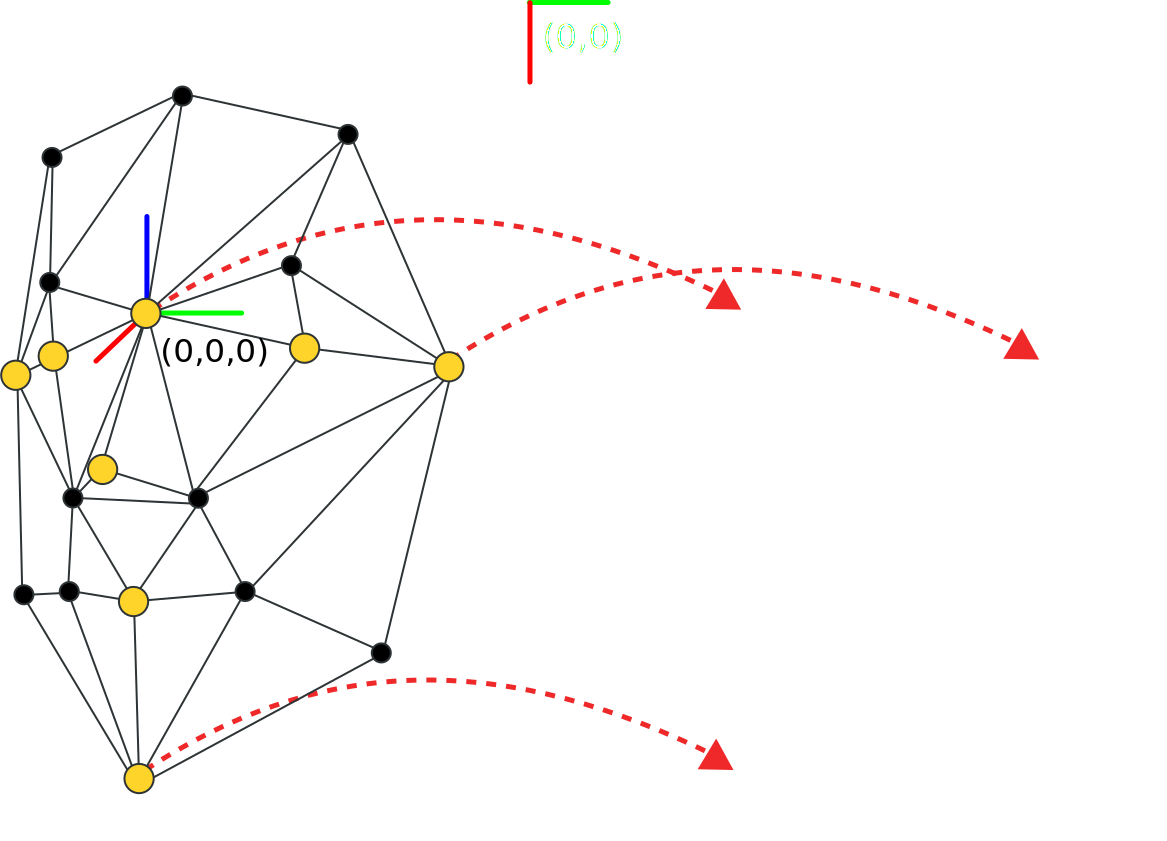
\includegraphics[width=0.9\linewidth]{head_pose}
    \caption{The 6D head pose is estimated by fitting a 3D model of an
        adult head (left) onto the detected 2D features of the face (right). We
        rely on an iterative $PnP$ algorithm, using 8 correspondence pairs
        (three are depicted: the sellion -- the nasal depression --, the left
        tragion and the menton). The 3D origin of the head is set at the sellion.}

    \label{head_pose}
\end{figure}

\begin{figure}[t]
    \centering
    
\includegraphics[width=\linewidth]{head_pose_real_world}
    \caption{Head pose results on images captured during a field experiment.
    Detection of face features (and therefore, estimation of the pose) is robust
    to significant occlusions and face rotations.}
    \label{head_pose_real_world}
\end{figure}

\subsection{Field \& Focus of Attention}

\begin{figure}
    \centering
    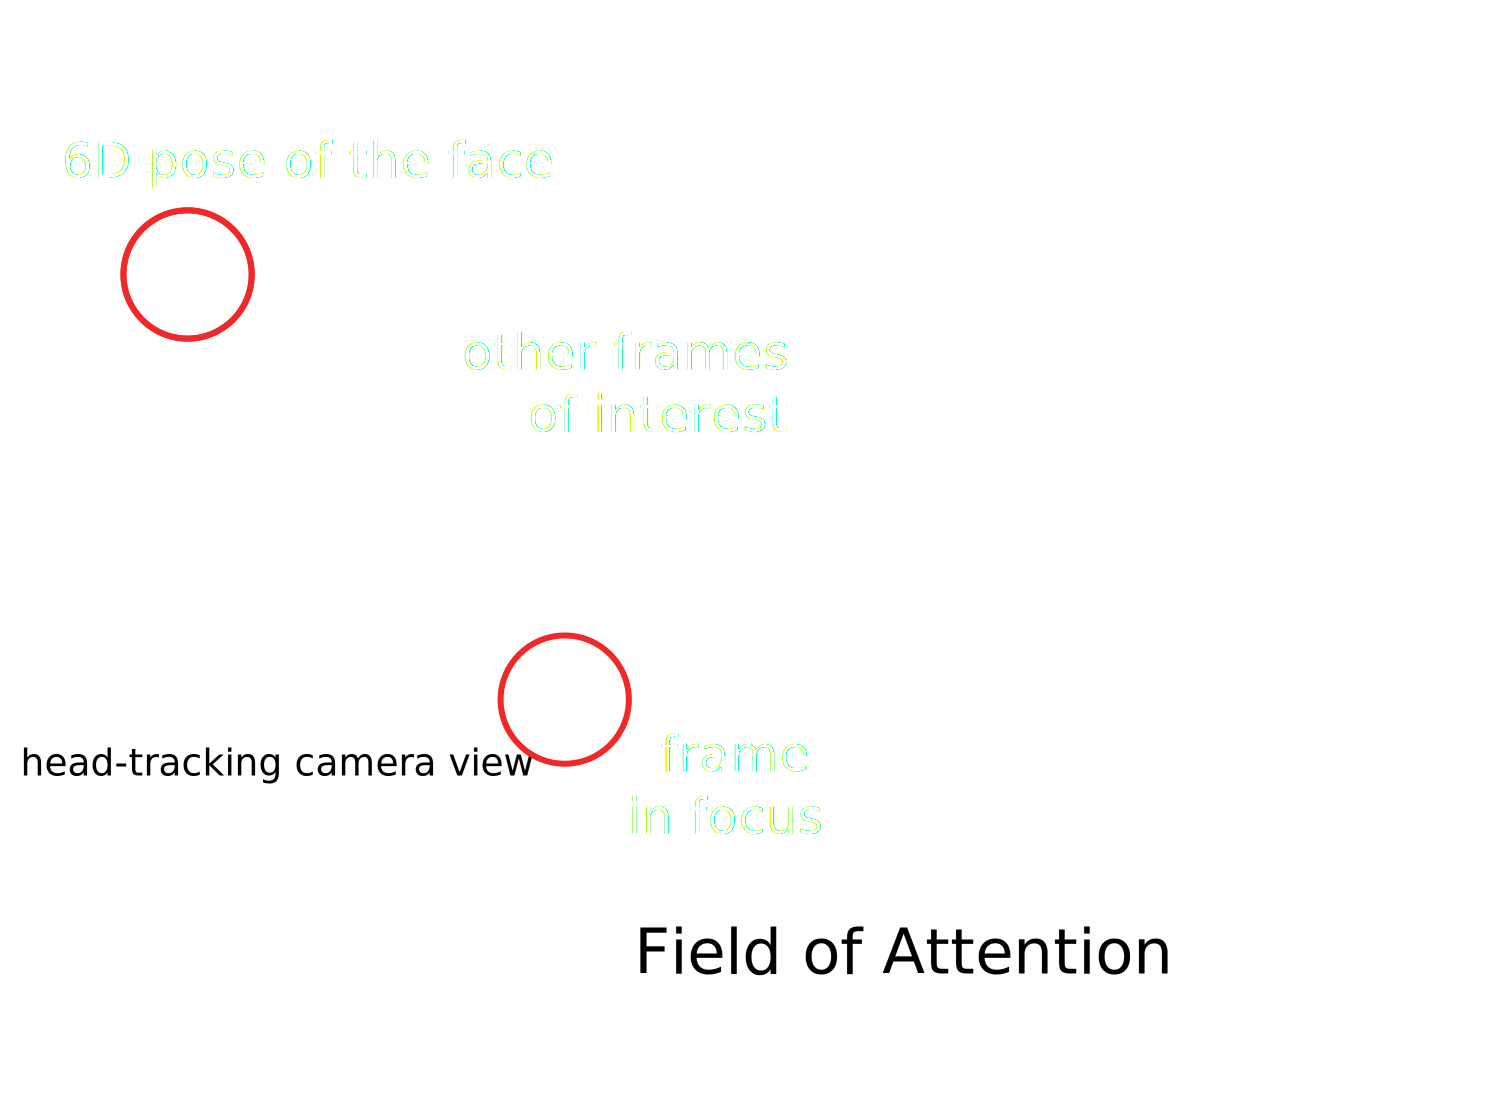
\includegraphics[width=0.9\columnwidth]{field_of_attention}
    \caption{\small The visual field of attention is approximated to a
        20$\degree$ cone, spanning from the head's sellion. The objects whose 3D
    pose intersect with this cone are considered \emph{in focus}.}
    \label{fig:vfoa}
\end{figure}

We model the field of attention as the central region of the field of view.
The field of view itself is approximated to a cone spanned from the nasal
depression (sellion) of the human face.

The width of the human field of attention has been discussed in the literature.
Holmqvist~\cite{holmqvist2011eye} specifies that the visual human
range\fixme{field of view or field of attention?} is $ \pm  40\degree $ in the
horizontal and $ \pm 25\degree $ in the vertical.
In~\cite{walker1980clinical}, Spector provides a more detailed specification
for each eye splitting the vertical range into $ 60\degree $ the upper region
and $ 75\degree $ the lower one. Moreover, the horizontal range gets separated
in $ 60\degree $ inwards (towards the nose) and $ 95\degree $ outwards.
Previous work on visual perspective taking for social robotics
application~\cite{sisbot2011situation} propose to use a cone of 30$\degree$ of
aperture. In the present implementation, the first approach explained has been
chosen representing the field of view using a cone with such
dimensions\fixme{which one? 40deg? 25deg?}.

We then approximate the visual focus of attention (VFoA) of the human to the
objects which lie inside the field of attention (Figure~\ref{fig:vfoa}). At a
given time, more than one object can therefore be \emph{in focus}.

Our implementation has two limitations: objects are approximated to their origin
(\ie objects are either in or out of the field of attention), and we do not
check actual visibility: one object could be hidden by another, it would still
be considered as in focus. We did not address these limitations since our
experimental setup (involving relatively small objects with no occlusions) did
not require it. Techniques for a more complete assessment of the visual
perspective can be found in~\cite{sisbot2011situation} for instance.

Within these limitations, computing if object $A(x_A,y_A,z_A)$ is in the field
of attention of the human requires first to transform the coordinates
$A(X_A,Y_A,Z_A)$ into the frame of the face, and then to verify the following
inequality (with $fov$ the aperture, and assuming that the main axis of the
field of attention is aligned on the face's $\vec{x}$):

\begin{align}
    \sqrt{Y_A^2 + Z_A^2} < tan\left(\frac{fov}{2}\right) \cdot X_A
\label{eq:fov}
\end{align}

Our approach assumes that the poses of the objects of interest are available to
the system: as described in section~\ref{sec:system}, our implementation relies
on the ROS {\sc tf} framework to manage and make available to all software
modules the list of poses of existing objects (represented as {\it frames}), and
dedicated perception modules are in charged of publishing up-to-date
informations regarding the location of the points of interest (the so-called
\emph{situation assessment}). Due to the nature of the experiment, most of the
points of interest considered for the experimental validation presented
hereafter are actually taken as static with respect to the robot.

%%%%%%%%%%%%%%%%%%%%%%%%%%%%%%%%%%%%%%%%%%%%%%%%%%%%%%%%%%%%%%%%%%%%%%%%%%%%%%%%%
%%%%%%%%%%%%%%%%%%%%%%%%%%%%%%%%%%%%%%%%%%%%%%%%%%%%%%%%%%%%%%%%%%%%%%%%%%%%%%%%%
%%%%%%%%%%%%%%%%%%%%%%%%%%%%%%%%%%%%%%%%%%%%%%%%%%%%%%%%%%%%%%%%%%%%%%%%%%%%%%%%%

\section{Experimental Validation}

As presented above, we use the (6D) head pose as an approximation of the
actual gaze direction, and we approximate from here the participant's field of
attention. The assumption that such an approximation of the field of attention
allows to derive the actual focus of attention is the core hypothesis that we
ought to validate.

This section presents such an experimental validation, set in the context of a
real child-robot interaction scenario where the robot tries to engage a child in
handwriting tasks using learning by teaching paradigm.

\paragraph{Real-Time Assessment of Visual Focus of Attention}

The participants' VFoA acquisition is the only dependent variable. This includes
their gaze times and patterns of looking or not looking to the targets. This
data extracted from an RGB camera was also coded post-hoc to quantify some of
these measurements.

We predict that there will be no generalizable pattern of participant's VFoA
behavior for different scenarios such as multiple subjects, necessitating in
situ VFoA estimation capabilities to enable robots to adapt in the specific
scenarios. However, we believe that off-line pattern identification can lead to
a better understanding of the children progression as well as engagement level
assessment in face-to-face long term interactions.\fixme{I did not understand
this paragraph}

\fixme{Underline difference between field of attention and focus of attention}

\fixme{State the hypothesis: head-pose estimation provides a good-enough
approximation of the gaze direction, and in turn of the field of attention, and
in turn of the focus of attention}


\subsection{Experimental Procedure}

The target of this study were 6 children with ages compressed between 5 and 6
years old. The experiments were developed individually and consisted on a
writing activity by turns and one story telling performed by the robot at a
given time of the interaction. All this performed in a over all 18 minutes
interaction average time.

Figure~\ref{fig:realSetup} illustrates our general experimental setup: a
face-to-face child-robot interaction with an (autonomous) Aldebran's {\sc nao}
robot.

\begin{figure}[h!]
    \centering
    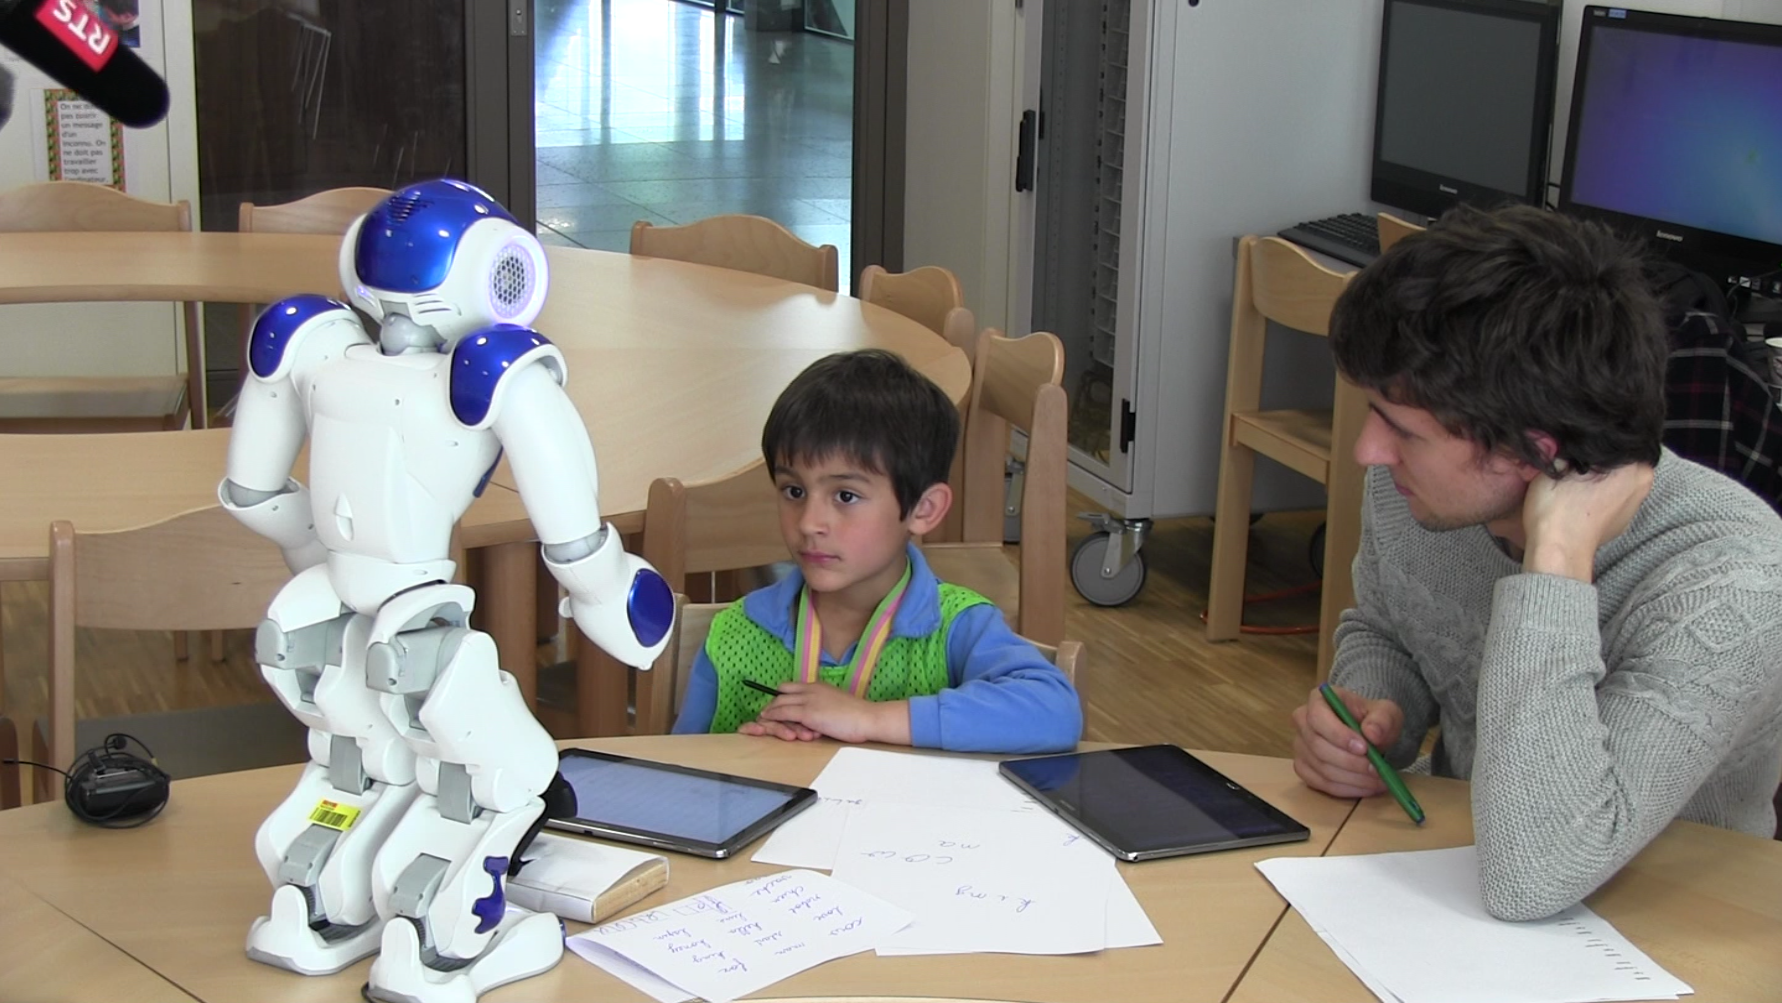
\includegraphics[width=1\columnwidth]{realSetup}
    \caption{\small Our experimental setup: face-to-face interaction with a {\sc
            nao} robot.  The robot writes on the tactile tablet, the child then
            corrects the robot by directly overwriting its letters on the tablet
            with a stylus. An adult (either a therapist or an experimenter,
            depending on the studies), remains next to the child to guide the work. 
            A second tablet allows to choose demonstrations and the camera captures the subject's face.}
    \label{fig:realSetup}
\end{figure}

A tactile tablet (with a custom application) is used for both the robot and the
child to write: during a typical round, the child requests the robot to write
something (a single letter, a number or a full word), and push the tablet
towards the robot, the robot writes on the tablet by gesturing the writing (but
without actually physically touching the tablet), the child then pull back the
tablet, corrects the robot's attempt by writing him/herself on top or next to
the robot's writing, and ``send'' his/her demonstration to the robot by pressing
a small button on the tablet. The robot ``learns'' from this demonstration and
tries again.

Since the child is assumed to take on the role of the teacher, we had to ensure
(s)he would be able to manage by him/herself the turn-taking and the overall
progression of the activity (moving to the next letter or word). In our design,
the turn-taking relies on the robot prompting for feedback once it is done with
its writing (simple sentences like ``What do you think?''), and pressing on a
small robot icon on the tablet once the child has finished correcting. In our
experiments, both were easy to grasp for children.

Implementing such a system raises several challenges that are discussed in
detail in \cite{Hood:2015}.

An RGB camera has been used to acquire images of 640x480 pixels at 25 fps. The
camera was located at 5 cm from the center of Nao's feet and its holder was tied
to a wood base for stability purposes. Thus, the camera's objective was 9 cm
above and $ 40\degree $ inclination with respect to the surface of the table to
maximize the detection during the writing time. However, Nao's camera could have
been used, always considering the \textit{tf} frame matrix update according to
the head orientation.

The subjects were typically located 50 cm away from the robot with the first
tablet in front and the second one 30 cm to the left of the first one. In the
same way, the experimenter was located around 60 cm to the left of the subject.
Finally, two observers were located far away from the interaction field to
manually assess the state of the interaction.

Figure \ref{drawSetup} allows us to intuitively identify several focuses of
attention along the interaction such as the two tablets, the robot, the
experimenter and the observers located in the diagonal.

\begin{figure}[h!]
    \centering
    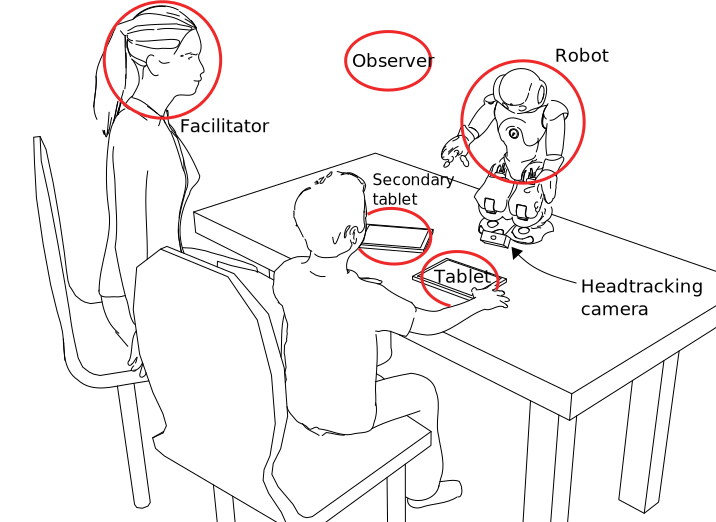
\includegraphics[width=0.8\columnwidth]{experimental_setup}
    \caption{\small \textbf{Experimental setting}. The areas of interest (AOI)
    of potential focuses of attention are circled in red.}
    \label{drawSetup}
\end{figure}

\subsection{System Implementation}
\label{sec:system}

\begin{figure}[h!]
    \centering
    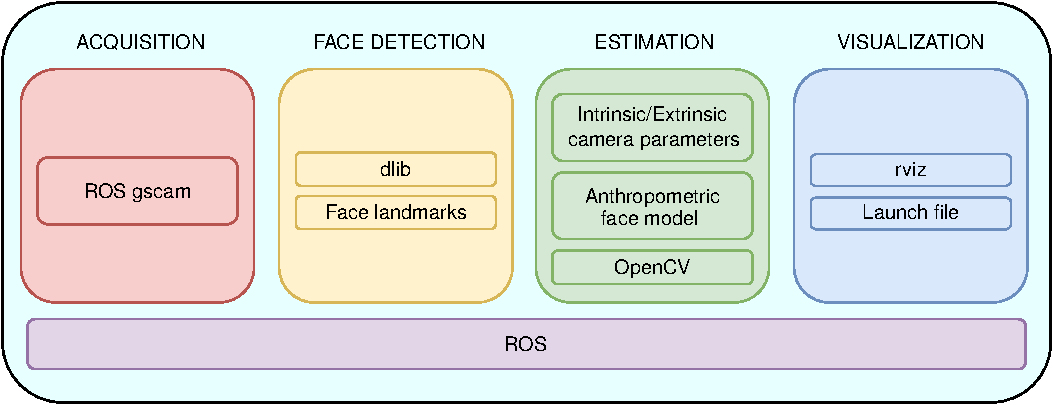
\includegraphics[width=0.9\columnwidth]{system}
    \caption{\small System overview showing the most relevant components involved in the estimation.}
    \label{system}
\end{figure}


, to detect and extract the skeleton
of the subject's face and then, use the obtained features to calculate the
head pose orientation estimation (see figure \ref{system}). In this way, we can
estimate what the subject was looking at and obtain an \textit{rviz} 3D scene
representation as it is executed as a ROS (Robot Operating System) node that can
be seen in figure \ref{rviz}. 

\subsection{Results}

\subsubsection{From Face Detection to Focus of Attention} \label{fromFaceTo}


Our results for a peer-to-peer work scenarios using an approach based on RGB
camera are summarized in table \ref{tab:results} where the \textit{expected} is
the focus of attention that given the state of the system, it is likely to
attract the subject's gaze. In the same manner, the \textit{captured} is the
focus of attention our approach provides and the \textit{real}, the ground truth
of the subject's gaze direction based on manual annotations from two evaluators
with an average reliability of $ \alpha = .89 $\fixme{Is that Cronbach alpha or
Krippendorff's alpha?}.

In order to calculate the inter-rater reliability between the two measurements
(real-captured and real-expected), the overlap percentage between the two
curves\fixme{which curve?}
has been computed. A more reliable measurement in terms of time shifting between
the real and captured focuses of attention is provided using the cosine
similarity\fixme{this needs to be better justified: why not a Cronbach alpha?} also shown in table~\ref{tab:results}. 

\begin{table*}[h!]
    \centering
    \caption{\textbf{Results of attention tracking accuracy}. \emph{Head pose
    tracking} is the percentage of total time of successful detection of the
    head pose; \emph{Ground-truth/robot match} is the percentage of matching time
    between manually annotated focus of attention (ground-truth) and robot's
    computed focus of attention.}

    \begin{tabular}{p{5.5cm}cccccccc}
        \toprule
        {\bf Subject} & 1 & 2 & 3 & 4 & 5 & 6 & {\bf Avg.} & {\it SD} \\
        \midrule
        {\bf Head pose tracking} (\%) & 88.2 & 83.5 & 90.5 & 83.1 & 87.9 & 85.0 & {\bf 86.4} & {\it 3.0} \\ 
        \midrule
        {\bf Ground-truth/robot match} (\%) & 61.1 & 85.5 & 80.8 & 62.2 & 63.4 & 83.9 & {\bf 72.8} & {\it 11.7}\\
        {\bf Cronbach's $\alpha$} &  & & & & & & & \\
        {\bf Cosine affinity} & 0.73 & 0.82 & 0.87 & 0.73 & 0.77 & 0.89 & {\bf 0.8} & {\it 0.07} \\
        \bottomrule
    \end{tabular}
    \label{tab:results}
\end{table*}


The results has proved that the VFoA prediction accuracy in the tracking is not
only conditioned by the subject's amount of movement, but also by the speed of
the same movements: Restless children externalize greater levels of movement
decreasing the VFoA prediction accuracy. 

For instance, subjects 1,4 and 5 despite the fact that the tracking accuracy is
in the average, the bad precision in the captured VFoA suggests that such
children are highly likely to modify the gaze direction without head move
intervention reducing dramatically the overlap between captured and real VFoA.

Additionally, several recurrent computer vision challenges such as the lighting
conditions, occlusions with the hands and the face angle with respect to the
camera, looking to the experimenter for instance, are factors that contribute to
reduce the tracking accuracy.

\subsubsection{Subject's Focus of Attention Analysis}

\begin{figure*}
    \centering
    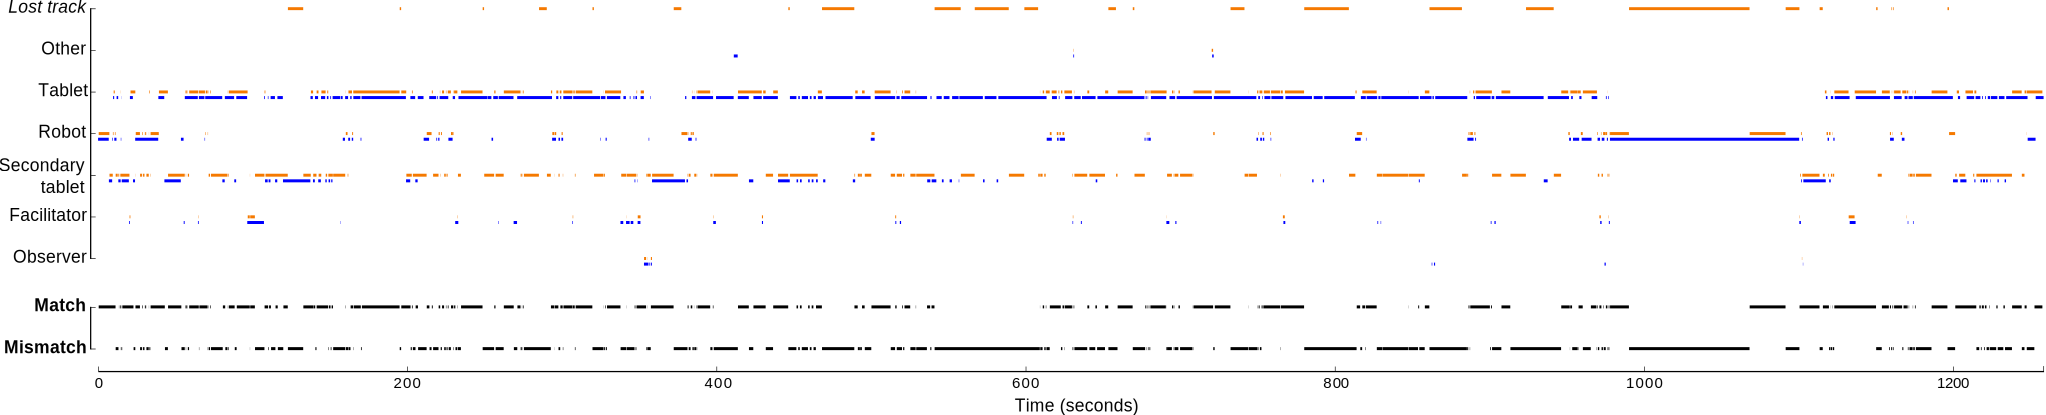
\includegraphics[width=\linewidth]{matches}
    \caption{\small \textbf{Comparison of computed focus of attention \vs ground
        truth} during a 20+ min face-to-face child-robot interaction (subject 4
        in table~\ref{tab:results}).
        In blue (top line), the focus of attention as computed by the robot;
        in orange (bottom line), the focus of attention as manually annotated
        (ground truth). The bottom graph shows agreements.}

    \label{fig:realExpected}
    
    % Maybe we should add the expected VFoA
\end{figure*}

According to figure \ref{fig:realExpected} several findings can be analyzed in
detail. The matching curve (cyan color) shows the overlapping between the
expected and the real focuses of attention. As can be noticed there is a
fluctuation at the beginning of the interaction as well as just before the
activity switching. These chaotic gaze manifestation is what we call an
automatic discovery of events, when the user experiences an uncertainty in the
present situation. 

The first one of the previous two situations presented above is due to the
novelty effect the subjects experience for the first time in front of the system
and according to the rest of participants suggests that the adaptation time is
around the first 2 minutes of interaction. In the second case, an unexpected
robot behavior produces such reaction due to an activity switching, the story
telling.

It is important to consider that in some occasions during the interaction, none
of the focuses of attention were within the field of view due to the time
transition from one focus to another resulting in an ambiguity. In order to deal
with these few cases it is assumed that the minimum distance between the height
of the field of view (cone) and the targets corresponds to the most likely focus
of attention. However, we also want to distinguish such cases when the subject
is directly not looking where the defined targets are located, but towards a
region far from the interaction field. These cases are not common but they can
be easily identified by setting a horizontal threshold to the field of view.

\begin{figure}[h!]
    \centering
    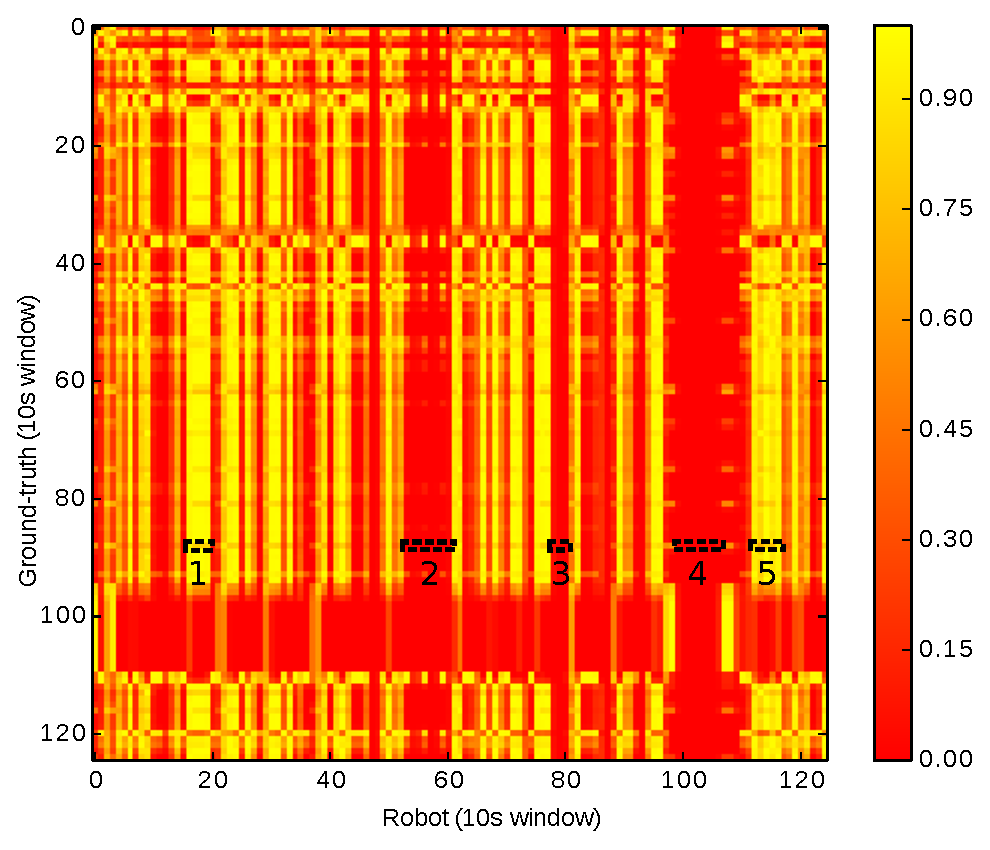
\includegraphics[width=0.7\columnwidth]{bitmap}
    \caption{\small Cosine similarity matrix between real and cap-tured VFoA
    using a 10 sec. window size computation. The correspondent numbers are shown
    in figure \ref{fig:realCaptured}.}
    \label{fig:bitmap}
\end{figure}

A relevant trend that can be observed is the continuous `look for approval'
situation where the subjects look at the experimenter in order to provide
feedback about the robot's response before providing their own one (see yellow
boxes in figure \ref{fig:realExpected}). Such transition tablet-experimenter
becomes more frequent in several cases, for instance when the experimenter makes
a suggestion (orange box in figure \ref{fig:realExpected}), in this case, switch
to a more complicated word.

Once the turn-taking is established, a pattern becomes visible during the
subject's feedback, when an attempt is performed: Such pattern shows a high
intermittent gaze frequency from the tablet to the selection. It also reveals
that the subject is using the demonstration model in the selection tablet to
provide a better answer to the robot. In fact, subjects decrease the response
time after each shift as well as the gaze frequency towards the model suggesting
an assimilation over time. Moreover, when a new demonstration is selected for
playing, the same behavior is replicated (see yellow boxes in figure
\ref{fig:realExpected}).

\subsubsection{Focus of attention distribution}

Additional information of the head pose can be obtained for the evaluation of
the VFoA distribution. Figure \ref{fig:heatmap} shows the most salient focuses
of attention where the peaks are located. These peaks are mainly projected
between the triangle composed by the robot, the writing tablet and the selection
tablet using an unsupervised K-means clustering method reveals, considering the
observers as negligible VFoA.

% Workaround to do subfigure since the packege looks not to work
\begin{figure}[th!]
  \centering
  \begin{tabular}{@{}c@{}}
    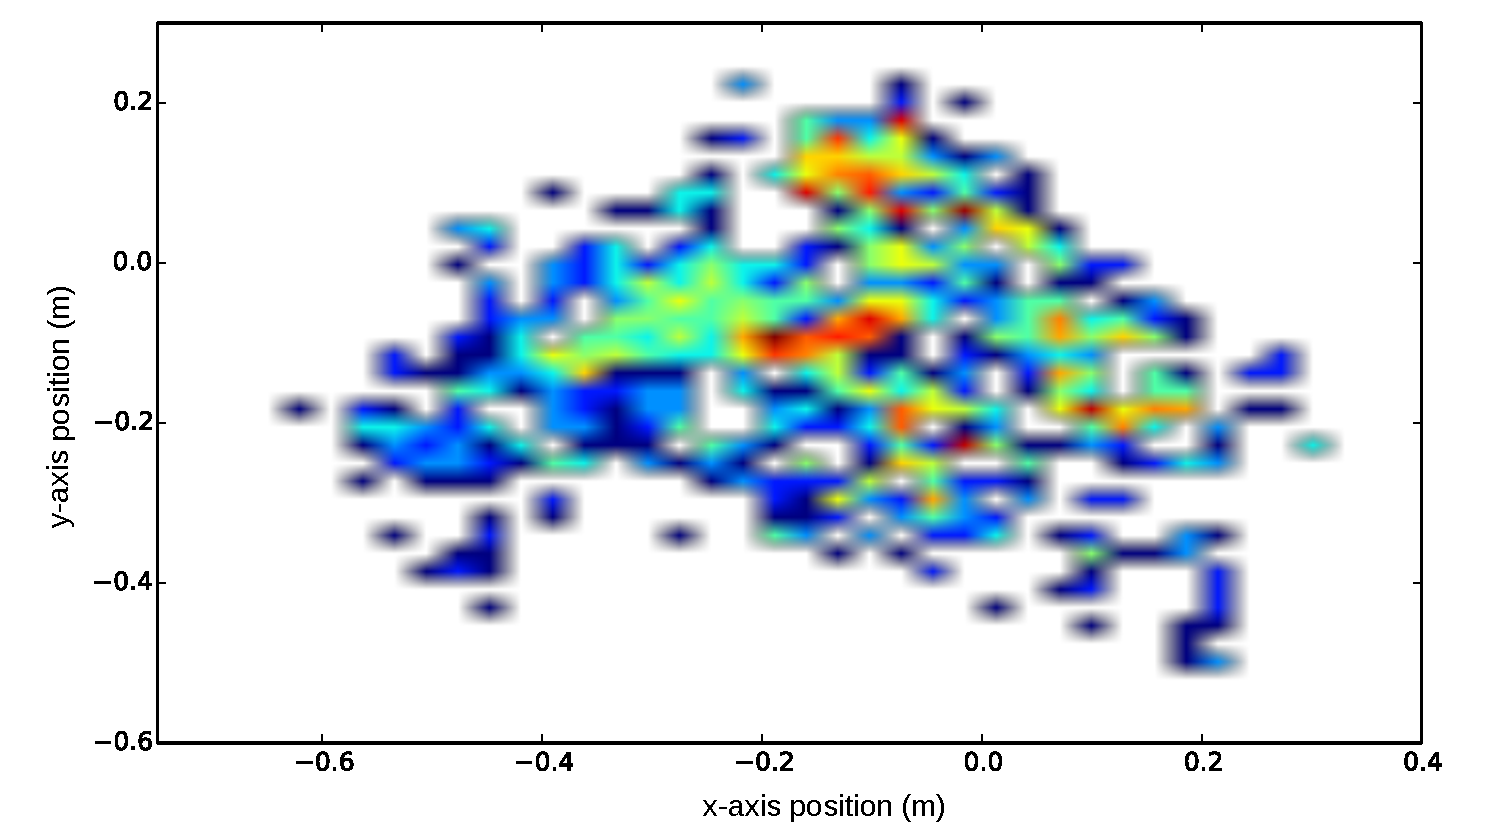
\includegraphics[width=.7\linewidth,height=100pt]{heatmap} \\
    \small (a)  2D histogram.
  \end{tabular}

  \vspace{\floatsep}

  \begin{tabular}{@{}c@{}}
    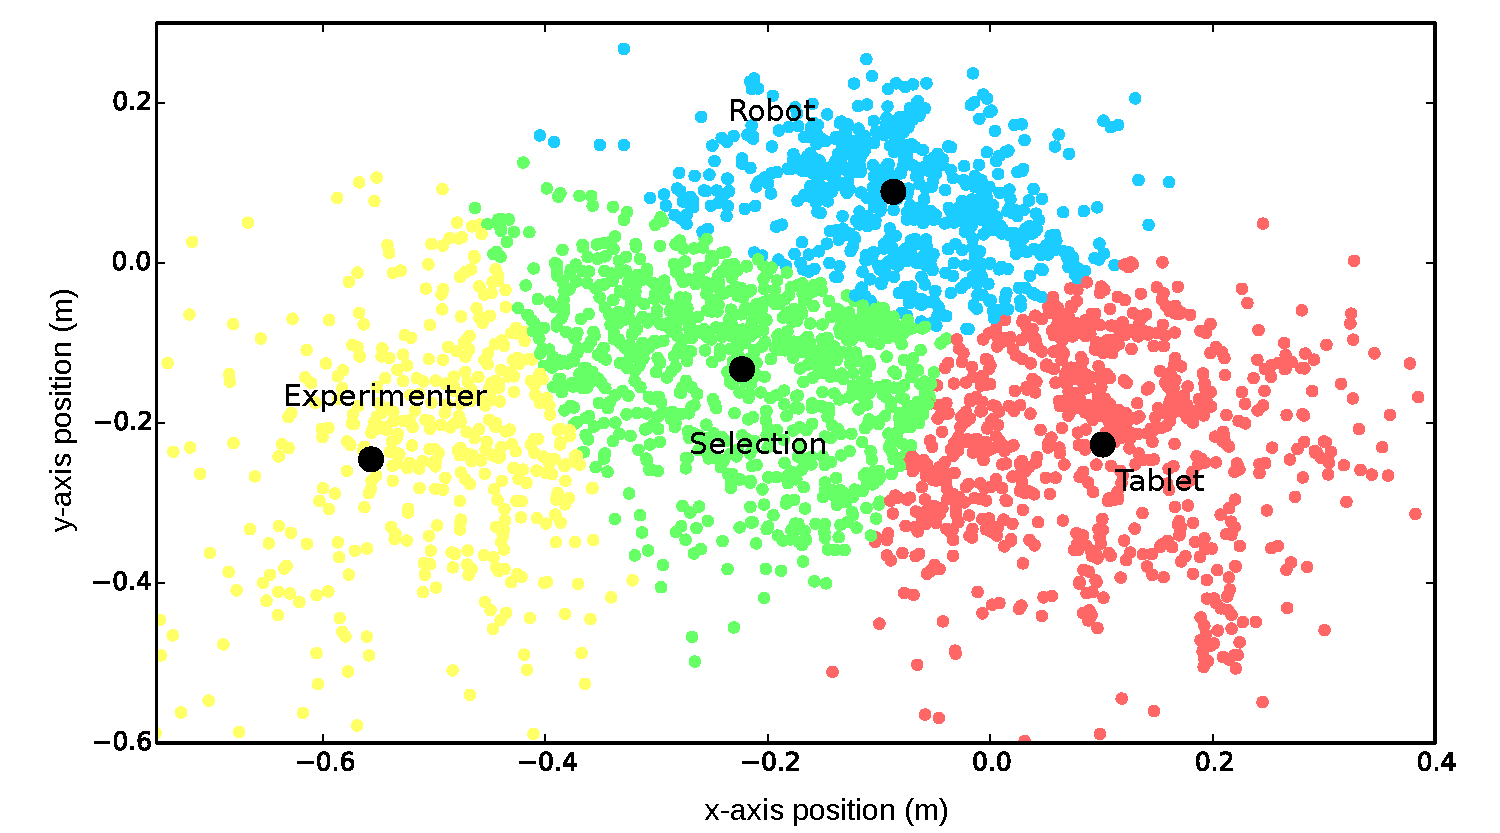
\includegraphics[width=.7\linewidth,height=100pt]{kmeans} \\
    \small (b) K-means clustering.
  \end{tabular}

  \caption{ \small Subject 4 head movements. (head yaw on x-axis, pitch on y-axis).}
  \label{fig:heatmap}
\end{figure}



%%%%%%%%%%%%%%%%%%%%%%%%%%%%%%%%%%%%%%%%%%%%%%%%%%%%%%%%%%%%%%%%%%%%%%%%%%%%%%%%%
%%%%%%%%%%%%%%%%%%%%%%%%%%%%%%%%%%%%%%%%%%%%%%%%%%%%%%%%%%%%%%%%%%%%%%%%%%%%%%%%%
%%%%%%%%%%%%%%%%%%%%%%%%%%%%%%%%%%%%%%%%%%%%%%%%%%%%%%%%%%%%%%%%%%%%%%%%%%%%%%%%%

\section{With-me-ness}

The concept of \emph{with-me-ness} has been introduced in the field of
\emph{Computer Supported Collaborative Learning} (CSCL) by Sharma~\etal
in~\cite{sharma2014me}. Sharma~\etal introduce this concept in an attempt to
answer a recurrent teacher's question: {\it ``how much are the students with
me?''}. They distinguish what they call \emph{perceptual with-me-ness} (the
student follows what the teacher refers to with deictic gestures) from
\emph{conceptual with-me-ness} (the student follows what the teacher refers to
verbally), and they show in an eye-tracking study that \emph{conceptual
with-me-ness} in particular correlates with better learning performance. This
also relates to the concept of gaze cross-recurrence that has been shown to
reflect the quality of the interaction~\cite{jermann2012effects} in
collaborative learning tasks.

Sharma~\etal simply define \emph{conceptual with-me-ness} as the normalized
percentage of time during which the student's gaze overlapped the areas of
teaching slides currently referred to by the teacher.
In order to apply it to human-robot interactions, we propose to extend this
concept, and to define \emph{conceptual with-me-ness} as the normalized
ratio of time that the human interactant focuses its attention on the
attentional target expected by the robot for the current task (or sub-task).


\begin{algorithm}[h!]
    \centering

    \begin{algorithmic}[1]
    \Procedure{Compute With-me-ness} {}
    \State $d_w, d_e \gets 0$
    \State $t \gets t_{start}$
    \Repeat
    \If{$task(t) \neq$ nil \textbf{and} \par
    \hskip\algorithmicindent$F(task(t)) \neq \varnothing$ \textbf{and} \par
    \hskip\algorithmicindent $f(t) \neq$ nil } \label{algline:skiplosttrack}
    \If{$f(t) \in F(task(t))$}
            \State $d_w \gets d_w + 1$
        \EndIf
        \State $d_e \gets d_e + 1$
    \EndIf
    \State $t \gets t + 1$
    \Until{$t = t_{end}$}

    \State $\mathcal{W}_{[start, end]} \gets \frac{d_w}{d_e}$
    \State \Return $\mathcal{W}_{[start, end]}$
    \EndProcedure

    \end{algorithmic}

    \caption{\textbf{Computation of \emph{with-me-ness}}. $d_w$ stands for the duration
        the human is \emph{with} the robot, $d_e$ stands for the duration where
        the human would be \emph{expected to be with} the robot, $task(t)$
        represents the task performed by the robot at time $t$ (possibly none),
        $F(task)$ represents the (possibly empty) set of expected attentional
        targets associated to task $task$, $f(t)$ represents the actual focus of
        attention measured at time $t$. $\mathcal{W}_{[start, end]}$ represents
        the level of \emph{with-me-ness} from $t_{start}$ to $t_{end}$.}
    \label{alg:with-me-ness}
\end{algorithm}

Algorithm~\ref{alg:with-me-ness} provides a formal way of computing the level of
with-me-ness $\mathcal{W}$ between two time points $[t_{start}, t_{end}]$. A
notable difference with the original definition by Sharma~\etal is that, at a
given time $t$, the task $task(t)$ performed by the robot may elicit more than
one attentional target; thus, at a given time, more than one location can be
regarded as possible \emph{expected} focuses of attention for the human. For
example, a robot which is writing, could typically elicit gazes to its hand as
well as to its head. A human looking at either of these locations would be
considered to be \emph{with} the robot in terms of interaction. Also notable, we
exclude from the computation of $\mathcal{W}$ all of the periods of time where
the user's focus of attention can not be estimated (Algorithm~\ref{alg:with-me-ness},
line~\ref{algline:skiplosttrack}, third condition), typically because the user's
face is not visible at those times.

\begin{table}[h!]
    \centering
    \caption{\textbf{Levels of with-me-ness}. For each subject, the with-me-ness level is reported over the whole interaction.}
    \begin{tabular}{p{2cm}cccccccc}
        \toprule
        \textbf{Subject} & 1 & 2 & 3 & 4 & 5 & 6 & Avg. & SD \\
        \midrule
        %Ground-truth \vs expected (\%) & 92.6 & 88.8  & 95.8 & 93.1 & 96.5 & 89.6 & 92.7 & \\ \hline
        $\mathcal{W}_{groundtruth}$ &  & & & & & & & \\ 
        {\it Cronbach's $\alpha$} &  & & & & & & & \\
        \midrule
        $\mathcal{W}_{robot}$ &  & & & & & & & \\
        {\it Cronbach's $\alpha$} &  & & & & & & & \\
        \bottomrule
    \end{tabular}
    \label{tab:results-with-me-ness}
\end{table}


\begin{figure*}
    \centering
    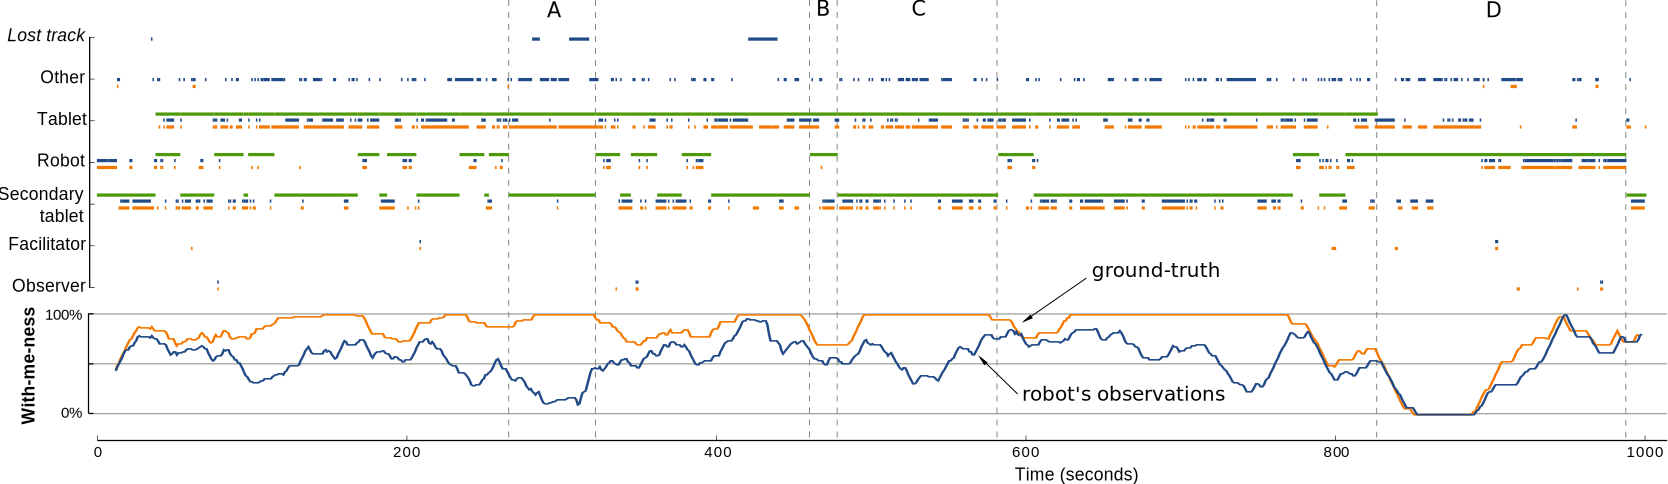
\includegraphics[width=\linewidth]{with-me-ness}
    \caption{\small \textbf{With-me-ness}. Evolution of the level of
    \emph{with-me-ness} over a 20min long child-robot interaction. The diagram
    is identical to Figure~\ref{fig:realExpected} with the \emph{expected}
    attentional targets added in green. The bottom curves represent the levels
    of with-me-ness (since the beginning of the interaction), computed following
    Algorithm~\ref{alg:with-me-ness}. The blue line is with-me-ness as estimated by
    the robot, the orange line is with-me-ness computed from manually annotated
    focuses of attention. The ``holes'' in the with-me-ness computed by the
    robot correspond to period of time where the child's face is not detected.}

    \label{fig:with-me-ness}
\end{figure*}

If we consider the case shown in section \ref{fromFaceTo}, evaluating the
subject's progression together with the time on task may be an indicator of
engagement: If the subject answers so quickly with respect to the previous
attempts with a poorer handwriting may be the case she is not engaged anymore.
In such hypothetical case an activity switch can be easily implemented in a
robot architecture. It confirms the findings reported in \cite{anzalone} where
time response to event is proposed to account quality of interaction. 

However, a high amount of gaze shift (figure \ref{fig:gazeR}) towards the
demonstration provided can reveal that the challenge is too big or no gaze, the
exactly the opposite. In this case, the robot response can be adapted to the
situation. Similar, but least relevant results are obtained using the
correctness (figure \ref{fig:errorR}) of the child's feedback after each
attempt. 

\begin{figure}
  \centering
  \begin{tabular}{@{}c@{}}
    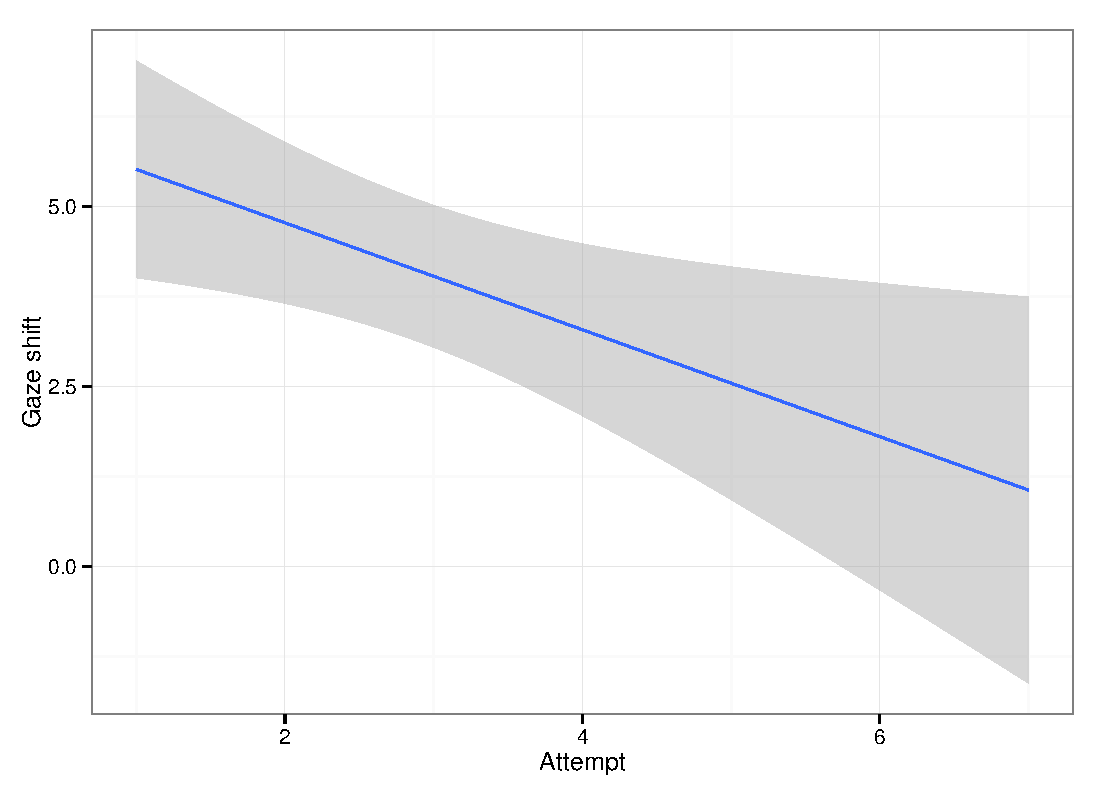
\includegraphics[width=.7\linewidth,height=100pt]{gazeR} \\
    \small (a) Occurrences of a gaze shift.
  \end{tabular}\label{fig:gazeR}

  \vspace{\floatsep}

  \begin{tabular}{@{}c@{}}
    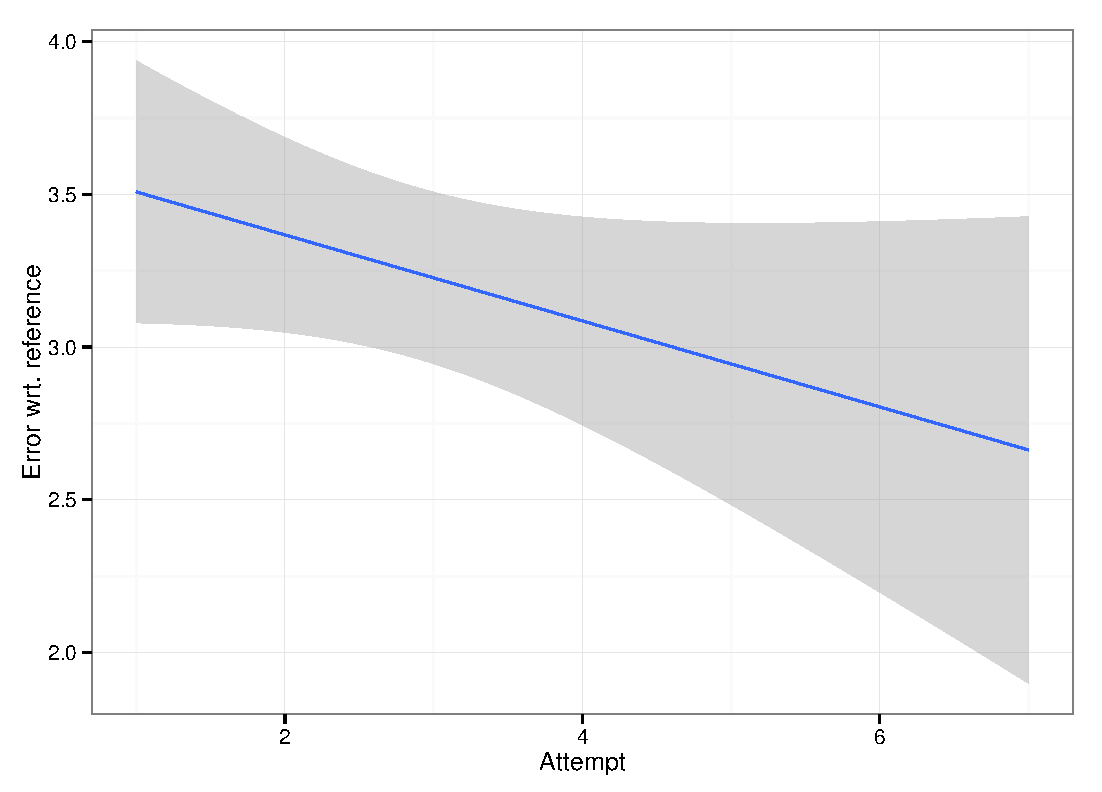
\includegraphics[width=.7\linewidth,height=100pt]{errorR} \\
    \small (b) Word correctness.
  \end{tabular}\label{fig:errorR}

  \caption{ \small Linear regression of all subject attempts against the gaze
  shift tablet-model (a) and the correctness as the average euclidean distance
  of each letter in its corresponding eigenspace with respect to a reference
  letter (b). The gray region defines the confidence interval.}
  
\end{figure}


This information can be used to estimate the child's state during the
interaction. For instance, if we consider that a low level of engagement is
produced by extremely high or low demanding situations, it is possible to assess
the engagement level during the interaction based on gaze shift and word
correctness.

It is also important to notice that the initiative of the robot into the
learning process in a turn-taking activity produces an effect in the engagement
of the human partner. However, experience suggests that a robot that learns
evoke a positive action in the partner. But the opposite, a robot that is not
able to progress over time, produces the contrary effect.

%Finally, the subjects set their attention more often to the tablet displaying the generated hand-writing during the robot feedback rather than to the robot itself. 

%%%%%%%%%%%%%%%%%%%%%%%%%%%%%%%%%%%%%%%%%%%%%%%%%%%%%%%%%%%%%%%%%%%%%%%%%%%%%%%%%
%%%%%%%%%%%%%%%%%%%%%%%%%%%%%%%%%%%%%%%%%%%%%%%%%%%%%%%%%%%%%%%%%%%%%%%%%%%%%%%%%
%%%%%%%%%%%%%%%%%%%%%%%%%%%%%%%%%%%%%%%%%%%%%%%%%%%%%%%%%%%%%%%%%%%%%%%%%%%%%%%%%


\section{Discussion and Conclusion}

In this work we have presented an on-line vision-based engagement assessment
solution that can be extended to work in different platforms for simulating
complex interaction scenarios monitoring several VFoA with a maker-less
technology. It provides some benefits like the decrement of the system
complexity as well as the increment of the naturalness of the interaction due to
the use of an RGB sensor.  

Furthermore, although it has not been tested in a real scenario with several
subjects at the same time, the approach also allows to handle such situations
too.

During the case study, results show that it is possible to distinguish between
long and short feedback episodes based on the gaze shift and depending on the
previous attempts performed by the subject. As a result, gaze-shift together
with the number of attempts becomes a reliable indicator candidate in the
assessment of the engagement during the activity.

Additionally, both the gaze shift and the correctness of the feedback seem to be
strictly correlated with the learning gain during the activity as they go in
decrement after each attempt provided by the subjects. Despite the fact that
these results are encouraging, there is a need of validation with a greater
amount of subjects.

Regarding to the approach used, some limitations need to be considered. The most
relevant one, the fact that the positions of the VFoA need to be known in
advance and defined as static \textit{tf} frames in the system. Moreover, it is
important to notice that eye gaze information is neglected which induces a
certain amount of error, as well as the noise induced by the 3D pose estimation
computed from face features.

Besides, our approach does not account for visual occlusions when computing the
focus of attention: any frame within the cone of the visual field of attention
is considered as \emph{in focus}. In reality, some of the frames may be visually
occluded and thus not seen by the subject. Computing actual visibility requires
more general situation assessment capabilities, and in particular (approximate)
3D models of the surrounding objects so that visibility testing may be
performed, as done in~\cite{sisbot2011situation} for instance. Our experimental
setting did not lead to any specific visual occlusions, and we did not developed
this capability.

Compared to intrusive hardware like head mounted
displays, eye-trackers or wearables for instance, this approach has a clear
advantage of simplicity and integration with robotic systems, but also becomes
accurate enough for general purposes in face-to-face interactions. In addition,
it allows us to model complex environments, handling different number and
positions of participants in the scene.

In that regards, it is interesting to put this work on human-robot interaction
in perspective with previous research conducted on ape-human interaction by
Tomasello~\etal~\cite{tomasello2007reliance}: they show that apes rely primarily
on the head pose to estimate the focus of attention of a human partner, in to contrast
to human children who primarily rely on eye direction. From this perspective,
our robot mimics attention tracking mechanism comparable to the ones found in apes.

Gaze information acquired during the interactions is not only useful to detect
and predict engagement, but also allows the possibility to develop actively the
concept gaze-aware robot. In other words, make the system able to estimate where
the subject looks at, but also imitate the same subject's VFoA when the activity
state allows it. 

%ACKNOWLEDGMENTS are optional
\section*{Acknowledgments}

This research was partially supported by the Funda\c{c}\~{a}o para a Ci\^{e}ncia
e a Tecnologia (FCT) with reference UID/CEC/ 50021/2013, and by the Swiss
National Science Foundation through the National Centre of Competence in
Research Robotics.

\bibliographystyle{abbrv}
\bibliography{sigproc}
\end{document}
